\chapter{Potencia y radicación}

En el capítulo anterior introdujimos el producto a partir de una situación particular: sumar varias veces el mismo número. Así, en los números naturales,
\[
4\cdot2=2+2+2+2.
\]

Ahora podemos hacer una pregunta semejante. ¿Qué ocurre cuando, en lugar de sumar varias veces el mismo número, lo multiplicamos varias veces por sí mismo? Por ejemplo,
\[
2\cdot2\cdot2\cdot2.
\]
Podemos evaluar este producto paso a paso y obtener \(16\). Sin embargo, la expresión también contiene otra información: el \(2\) es el factor que se repite y aparece cuatro veces. La escritura
\[
2^4
\]
permite conservar esa estructura de manera breve.

La operación que representa un producto de factores iguales recibe el nombre de \emph{potenciación}. Como ocurrió con el producto, comenzaremos en un caso sencillo y luego ampliaremos gradualmente su significado. Esa ampliación nos conducirá a exponentes negativos, raíces y exponentes racionales.

\section{La potencia como producto repetido}

Considere nuevamente el producto
\[
2\cdot2\cdot2\cdot2.
\]
Como los cuatro factores son iguales, podemos abreviarlo mediante
\[
2^4.
\]
Por lo tanto,
\[
2^4=2\cdot2\cdot2\cdot2=16.
\]
Las tres escrituras representan el mismo número, pero muestran aspectos diferentes. La primera hace visibles los factores; la segunda señala directamente qué factor se repite y cuántas veces; la tercera es el numeral obtenido al evaluar la expresión.

\begin{definitionbox}[Potencia con exponente natural positivo]
Sean \(a\in\mathbb N\) y \(n\in\mathbb N\) con \(n>0\). Se define
\[
a^n=
\underbrace{a\cdot a\cdot\ldots\cdot a}_{n\text{ factores}}.
\]
El número \(a\) recibe el nombre de \emph{base}; el número \(n\), el de \emph{exponente}; y el valor de la expresión completa, el de \emph{potencia}.
\end{definitionbox}

Por ejemplo, en
\[
3^5=3\cdot3\cdot3\cdot3\cdot3=243,
\]
la base es \(3\), el exponente es \(5\) y la potencia es \(243\).

La posición de cada número es parte de la notación. La base indica cuál es el factor repetido; el exponente indica cuántas veces aparece. Por eso, en general, intercambiarlos modifica la cantidad representada:
\[
2^3=2\cdot2\cdot2=8,
\qquad
3^2=3\cdot3=9.
\]
No existe una propiedad conmutativa de la potenciación: normalmente \(a^n\ne n^a\).

\subsection{Exponente uno}

Si el exponente es \(1\), la base aparece como factor una sola vez. En consecuencia,
\[
a^1=a.
\]
No es necesario imaginar un producto de varios factores: la expresión \(a^1\) representa simplemente el mismo número que \(a\).

\subsection{Exponente cero}

La definición como producto repetido nos permite entender las potencias con exponente positivo. También muestra una relación sencilla entre potencias consecutivas.

Por ejemplo,
\[
2^4
=2\cdot2\cdot2\cdot2
=(2\cdot2\cdot2)\cdot2
=2^3\cdot2.
\]
Del mismo modo,
\[
2^3=2^2\cdot2,
\qquad
2^2=2^1\cdot2.
\]

En general, aumentar el exponente en una unidad equivale a agregar un factor igual a la base:
\[
a^{n+1}=a^n\cdot a,
\qquad n>0.
\]
Esta igualdad no es una nueva regla que debamos memorizar; se obtiene directamente de la definición de potencia como producto repetido.

Ahora queremos extender la notación para incluir el exponente \(0\). Para hacerlo de manera compatible con la relación anterior, debería cumplirse también
\[
a^1=a^0\cdot a.
\]
Pero ya sabemos que
\[
a^1=a.
\]
Por lo tanto,
\[
a=a^0\cdot a.
\]

Si \(a\ne0\), podemos dividir ambos lados entre \(a\):
\[
\frac{a}{a}
=
\frac{a^0\cdot a}{a},
\]
y obtenemos
\[
1=a^0.
\]

Esto nos conduce a la siguiente definición.

\begin{definitionbox}[Potencia con exponente cero]
Para todo número \(a\ne0\), se define
\[
a^0=1.
\]
\end{definitionbox}

La condición \(a\ne0\) es importante. Si intentáramos hacer el mismo razonamiento con base cero, la relación
\[
a^1=a^0\cdot a
\]
se convertiría en
\[
0=0^0\cdot0.
\]
Pero esta igualdad se cumple cualquiera sea el valor colocado en lugar de \(0^0\), ya que todo número multiplicado por cero da cero. Por lo tanto, este razonamiento no determina un valor para \(0^0\).

En este libro dejaremos \(0^0\) sin definir. En contextos más avanzados puede asignársele algún valor por conveniencia, pero esa elección depende del contexto.

En cambio, cuando el exponente es positivo,
\[
0^n=0
\qquad(n>0),
\]
porque el producto contiene al menos un factor igual a cero.

\subsection{La base no tiene que natural}

Hasta ahora hemos utilizado principalmente números positivos como base, pero la idea de potencia como producto repetido también funciona cuando la base es negativa.

Por ejemplo,
\[
(-2)^3=(-2)\cdot(-2)\cdot(-2)=-8,
\]
mientras que
\[
(-2)^4=(-2)\cdot(-2)\cdot(-2)\cdot(-2)=16.
\]

La diferencia está en la cantidad de factores negativos.

Recordemos que el producto de dos números negativos es positivo:
\[
(-a)(-a)=a^2.
\]

Por eso, si tenemos una cantidad par de factores negativos, podemos agruparlos de dos en dos. Cada pareja produce un resultado positivo. Por ejemplo,
\[
(-2)^6
=
\bigl((-2)(-2)\bigr)
\bigl((-2)(-2)\bigr)
\bigl((-2)(-2)\bigr),
\]
y por lo tanto el resultado es positivo.

En cambio, si la cantidad de factores es impar, después de formar todas las parejas posibles queda un factor negativo sin pareja:
\[
(-2)^5
=
\bigl((-2)(-2)\bigr)
\bigl((-2)(-2)\bigr)
(-2),
\]
de modo que el resultado es negativo.

Este razonamiento no depende de cuántos factores haya. Siempre podemos agrupar los factores negativos de dos en dos. Por ello, para \(a>0\),
\[
(-a)^n=
\begin{cases}
a^n, & \text{si \(n\) es par},\\[4pt]
-a^n, & \text{si \(n\) es impar}.
\end{cases}
\]

No es necesario memorizar esta expresión: el signo puede determinarse simplemente observando si la cantidad de factores negativos es par o impar.

\begin{note}
  Mucho cuidado con expresiones como 
  \[
    -a^n
  \]
  ya que el signo \(-\) en tal caso no se considera parte de la potencia. Es decir, la interpretación es 
  \[
    - (a^n)
  \]
\end{note}

\subsubsection{Los paréntesis importan}

Cuando la base es negativa, los paréntesis permiten indicar que el signo forma parte de la base.

Por ejemplo,
\[
(-2)^4
\qquad\text{y}\qquad
-2^4
\]
representan expresiones diferentes.

En
\[
(-2)^4,
\]
la base es \(-2\), por lo que
\[
(-2)^4
=
(-2)(-2)(-2)(-2)
=
16.
\]

En cambio, en
\[
-2^4,
\]
la base de la potencia es \(2\). Primero se calcula
\[
2^4=16
\]
y luego se toma su opuesto:
\[
-2^4=-(2^4)=-16.
\]

Por lo tanto,
\[
(-2)^4=16,
\qquad
-2^4=-16.
\]

\subsection{Una fracción también puede ser la base}

La base de una potencia también puede ser una fracción. La interpretación sigue siendo exactamente la misma: elevar a un exponente natural positivo significa multiplicar la base por sí misma tantas veces como indica el exponente.

Por ejemplo,
\[
\left(\frac{2}{3}\right)^3
=
\frac{2}{3}\cdot
\frac{2}{3}\cdot
\frac{2}{3}.
\]

Como ya sabemos multiplicar fracciones, podemos multiplicar los numeradores entre sí y los denominadores entre sí:
\[
\left(\frac{2}{3}\right)^3
=
\frac{2\cdot2\cdot2}{3\cdot3\cdot3}
=
\frac{8}{27}.
\]

Observemos ahora la forma en que aparecen el numerador y el denominador:
\[
2\cdot2\cdot2=2^3,
\qquad
3\cdot3\cdot3=3^3.
\]
Por lo tanto,
\[
\left(\frac{2}{3}\right)^3
=
\frac{2^3}{3^3}.
\]

El mismo razonamiento funciona con cualquier fracción cuyo denominador sea distinto de cero. Si \(b\ne0\), entonces
\[
\left(\frac{a}{b}\right)^n
=
\frac{a^n}{b^n},
\qquad n>0.
\]

Esta igualdad no introduce una nueva manera de calcular potencias. Es simplemente lo que obtenemos al escribir la potencia como un producto repetido:
\[
\left(\frac{a}{b}\right)^n
=
\underbrace{
\frac{a}{b}\cdot
\frac{a}{b}\cdots
\frac{a}{b}
}_{n\text{ factores}}
=
\frac{
  \overbrace{a\cdot a\cdots a}^{n\text{ factores}}
}{
\underbrace{b\cdot b\cdots b}_{n\text{ factores}}
}
=
\frac{a^n}{b^n}.
\]

La fracción también puede ser negativa. Por ejemplo,
\[
\left(-\frac{2}{3}\right)^3
=
\left(-\frac{2}{3}\right)
\left(-\frac{2}{3}\right)
\left(-\frac{2}{3}\right)
=
-\frac{8}{27},
\]
mientras que
\[
\left(-\frac{2}{3}\right)^4
=
\frac{16}{81}.
\]

Nuevamente, el signo depende de la cantidad de factores negativos: un exponente par produce un resultado positivo y un exponente impar produce un resultado negativo.


\section[Propiedades de potencias naturales]{Propiedades de las potencias con exponentes naturales}

Algunas de estas propiedades ya fueron presentadas para introducir definiciones como \(a^0\). Sin embargo aquí se presentarán las propiedades generales.

Las propiedades de esta sección no son reglas aisladas. Todas pueden comprenderse escribiendo las potencias como productos y observando qué ocurre con sus factores.

\subsection{Producto de potencias de igual base}

Considere
\[
2^3\cdot2^4.
\]
Al desarrollar ambas potencias obtenemos
\[
(2\cdot2\cdot2)\cdot(2\cdot2\cdot2\cdot2).
\]
En total aparecen siete factores iguales a \(2\). Por lo tanto,
\[
2^3\cdot2^4=2^7=2^{3+4}.
\]
De manera general, si \(m,n\in\mathbb N\),
\[
a^m\cdot a^n=a^{m+n}.
\]
Si alguno de los exponentes es cero, se requiere \(a\ne0\), pues hemos definido \(a^0\) solamente para bases no nulas.

Observe qué cambia y qué se conserva: la base común permanece; los exponentes se suman porque estamos reuniendo dos grupos de factores iguales.

\subsection{Cociente de potencias de igual base}

Consideremos ahora el cociente
\[
\frac{3^5}{3^2}.
\]
Si desarrollamos las potencias como productos, obtenemos
\[
\frac{3^5}{3^2}
=
\frac{3\cdot3\cdot3\cdot3\cdot3}{3\cdot3}.
\]

Para comprender qué ocurre, podemos utilizar la regla de multiplicación de fracciones estudiada anteriormente y escribir el cociente como un producto:
\[
\frac{3\cdot3\cdot3\cdot3\cdot3}{3\cdot3}
=
\frac33\cdot
\frac33\cdot
\frac31\cdot
\frac31\cdot
\frac31.
\]

Los denominadores iguales a \(1\) no modifican el valor de los últimos factores. En cambio, los dos primeros cocientes valen \(1\):
\[
\frac33=1.
\]
Por lo tanto,
\[
\frac{3^5}{3^2}
=
1\cdot1\cdot3\cdot3\cdot3.
\]

Como \(1\) es el elemento neutro de la multiplicación,
\[
1\cdot1\cdot3\cdot3\cdot3
=
3\cdot3\cdot3
=
3^3.
\]
Así,
\[
\frac{3^5}{3^2}
=
3^3
=
3^{5-2}.
\]

Observe qué ha ocurrido. En el numerador había cinco factores iguales a \(3\), mientras que en el denominador había dos. Cada factor del denominador formó un cociente
\[
\frac33=1
\]
con uno de los factores del numerador. Como esos cocientes iguales a \(1\) no modifican el producto, permanecieron solamente tres factores iguales a \(3\).

Esta es la razón por la que aparece la resta de los exponentes.

El mismo razonamiento puede hacerse con cualquier base no nula. Si \(m>n\), podemos representar
\[
\frac{a^m}{a^n}
\]
como un producto que contiene \(n\) cocientes iguales a
\[
\frac aa=1
\]
y, además, \(m-n\) factores iguales a
\[
\frac a1=a.
\]
Por lo tanto, después de reemplazar los primeros por \(1\), permanecen \(m-n\) factores iguales a \(a\):
\[
\frac{a^m}{a^n}=a^{m-n}.
\]

Si los exponentes son iguales, no queda ningún factor de \(a\). En ese caso,
\[
\frac{a^n}{a^n}=1,
\]
y como ya hemos definido
\[
a^0=1
\qquad(a\ne0),
\]
también podemos escribir
\[
\frac{a^n}{a^n}=a^0=a^{n-n}.
\]

En consecuencia, para \(a\ne0\) y \(m,n\in\mathbb N\) con \(m\ge n\),
\[
\boxed{\frac{a^m}{a^n}=a^{m-n}}.
\]

La condición \(a\ne0\) es necesaria. El razonamiento utiliza cocientes de la forma
\[
\frac aa,
\]
que solamente valen \(1\) cuando \(a\ne0\). Además, necesitamos que el denominador de la expresión original sea distinto de cero.

También pedimos por ahora que
\[
m\ge n,
\]
de modo que \(m-n\) sea un exponente natural. Más adelante, cuando introduzcamos los exponentes negativos, podremos estudiar qué ocurre cuando \(m<n\).

\subsection{Potencia de una potencia}

En la expresión
\[
(2^3)^4,
\]
la base de la potencia exterior es la expresión completa \(2^3\). Desarrollarla significa repetirla como factor cuatro veces:
\[
(2^3)^4=2^3\cdot2^3\cdot2^3\cdot2^3.
\]
Cada grupo aporta tres factores iguales a \(2\), y hay cuatro grupos. En total aparecen \(3\cdot4=12\) factores:
\[
(2^3)^4=2^{12}=2^{3\cdot4}.
\]
Así, para exponentes naturales,
\[
(a^m)^n=a^{m\cdot n},
\]
siempre que las potencias que aparecen estén definidas.

\subsection{Potencia de un producto}

Considere
\[
(2\cdot3)^4.
\]
Al desarrollar la potencia,
\[
(2\cdot3)(2\cdot3)(2\cdot3)(2\cdot3).
\]
Por las propiedades asociativa y conmutativa del producto, podemos reunir los factores iguales:
\[
(2\cdot2\cdot2\cdot2)(3\cdot3\cdot3\cdot3)=2^4\cdot3^4.
\]
De manera general,
\[
(a\cdot b)^n=a^n\cdot b^n.
\]

También, si \(b\ne0\),
\[
\left(\frac ab\right)^n=\frac{a^n}{b^n}.
\]
Esta última igualdad se obtiene multiplicando \(n\) veces la fracción \(a/b\) y aplicando la regla del producto de fracciones como se demostró en la sección anterior.

\subsection{Poner a prueba las propiedades}

Hasta ahora hemos encontrado varias propiedades de las potencias observando cómo se comportan sus factores. Pero es razonable preguntarse hasta dónde llegan esas propiedades.

Por ejemplo, sabemos que
\[
2^3\cdot2^4=2^{3+4}.
\]
La explicación fue sencilla: al desarrollar ambas potencias aparecen tres factores iguales a \(2\) y otros cuatro factores iguales a \(2\). Al juntarlos obtenemos siete factores iguales:
\[
(2\cdot2\cdot2)(2\cdot2\cdot2\cdot2)
=
2^7.
\]

Pero entonces surge una pregunta natural:

\[
\text{¿qué ocurre si las bases son distintas?}
\]

Podríamos preguntarnos, por ejemplo, si es posible hacer algo semejante con
\[
2^3\cdot3^4.
\]

Cuando no estamos seguros de que una operación sea válida, no necesitamos memorizar una prohibición. Podemos formular lo que creemos que podría ocurrir y ponerlo a prueba.

Supongamos, por ejemplo, que intentáramos multiplicar las bases y sumar los exponentes:
\[
2^3\cdot3^4
\stackrel{?}{=}
(2\cdot3)^{3+4}.
\]

El símbolo \(\stackrel{?}{=}\) expresa precisamente nuestra duda: queremos averiguar si ambos lados son realmente iguales.

Calculemos cada uno por separado.

Por un lado,
\[
2^3\cdot3^4
=
8\cdot81
=
648.
\]

Por el otro,
\[
(2\cdot3)^{3+4}
=
6^7
=
279936.
\]

Como
\[
648\ne279936,
\]
la igualdad propuesta es falsa.

Esto nos permite comprender algo más importante que una regla: la propiedad
\[
a^m\cdot a^n=a^{m+n}
\]
funciona porque todos los factores tienen la misma base. Si las bases son diferentes, el razonamiento que dio origen a la propiedad ya no puede hacerse de la misma manera.

Podemos investigar otras dudas siguiendo el mismo procedimiento.

Por ejemplo, alguien podría preguntarse si una potencia puede distribuirse sobre una suma:
\[
(a+b)^n
\stackrel{?}{=}
a^n+b^n.
\]

No necesitamos aceptar ni rechazar la idea sin examinarla. Probemos con valores sencillos:
\[
a=2,\qquad b=3,\qquad n=2.
\]

Entonces, el lado izquierdo es
\[
(2+3)^2
=
5^2
=
25,
\]
mientras que el lado derecho es
\[
2^2+3^2
=
4+9
=
13.
\]

Obtuvimos
\[
25\ne13.
\]

Por lo tanto,
\[
(a+b)^n=a^n+b^n
\]
no puede ser una propiedad válida para todos los números.

Este tipo de ejemplo recibe el nombre de \emph{contraejemplo}. Cuando alguien afirma que una igualdad se cumple siempre, encontrar un solo caso en el que falle es suficiente para demostrar que la afirmación general es falsa.

Hay que tener cuidado con la situación inversa. Encontrar uno, diez o incluso cien ejemplos en los que una igualdad funciona no demuestra que funcionará siempre. Los ejemplos pueden ayudarnos a descubrir un patrón o a sospechar que una propiedad es cierta, pero una propiedad general necesita además una razón que explique por qué se cumple en todos los casos.

Esta distinción será útil durante todo el libro:

\begin{itemize}
    \item si sospechamos que una afirmación es falsa, podemos intentar encontrar un contraejemplo;
    \item si sospechamos que es verdadera, podemos probar algunos casos para comprenderla, pero después necesitaremos justificar por qué funciona siempre.
\end{itemize}

Las propiedades de las potencias no son instrucciones arbitrarias sobre qué símbolos pueden moverse. Cada una expresa algo que ocurre con los números y sus productos. Por eso, cuando aparezca una duda, siempre podemos volver a los significados que ya conocemos, desarrollar las operaciones y dejar que los propios números nos indiquen si nuestra idea puede ser correcta.

\begin{note}[title=\textbf{\color{teal}{Una pequeña pausa filosófica}}]

Hay algo curioso en lo que acabamos de hacer. Planteamos una pregunta matemática y, en cierto sentido, dejamos que las propias matemáticas respondieran.

Preguntamos si
\[
(a+b)^n=a^n+b^n
\]
podía ser siempre cierto. Después elegimos unos valores, seguimos las reglas que ya conocíamos y llegamos a una respuesta que no dependía de nuestra opinión: ambos lados dieron números distintos.

Esta es una de las características más fascinantes de las matemáticas. Nosotros formulamos las preguntas, inventamos símbolos, definiciones y formas de representar las ideas; pero, una vez que aceptamos ciertas reglas, no podemos decidir libremente cuáles serán sus consecuencias. Tenemos que descubrirlas.

Por eso existe una antigua discusión filosófica: ¿las matemáticas se inventan o se descubren?

En este libro adoptaremos una postura sencilla: un poco de ambas.

Podemos crear definiciones, elegir axiomas y construir nuevos sistemas matemáticos. Pero una vez establecidos esos puntos de partida, aparecen relaciones y consecuencias que ya no podemos escoger a nuestro gusto. Podemos explorarlas, intentar comprenderlas y descubrir hasta dónde nos llevan.

En ese sentido, aprender matemáticas no consiste solamente en aprender a manipular símbolos. También consiste en aprender a hacer preguntas y en escuchar las respuestas que surgen al seguir cuidadosamente la lógica.

A veces esas respuestas son inmediatas. Otras veces han requerido años, siglos o todavía no las conocemos.

Y quizá esa sea una de las razones por las que las matemáticas resultan tan profundas: comenzamos jugando con unas pocas ideas y, al seguir sus consecuencias, podemos terminar descubriendo estructuras y patrones que cambian nuestra manera de entender el mundo.
\end{note}

\subsection{Potencias y jerarquía de operaciones}

Al incorporar la potenciación necesitamos ampliar la convención de precedencia. Las potencias se consideran agrupadas antes que los productos, y los productos antes que las sumas. Así,
\[
3+2\cdot5^2
\]
se interpreta como
\[
3+\bigl(2\cdot(5^2)\bigr).
\]
Primero se evalúa \(5^2=25\), luego \(2\cdot25=50\) y finalmente \(3+50=53\).

Esta convención explica la diferencia entre
\[
-2^2=-(2^2)=-4
\]
y
\[
(-2)^2=4.
\]
En la primera expresión, el signo menos no pertenece a la base; en la segunda, los paréntesis indican que la base completa es \(-2\).

Como antes, la precedencia es una convención de escritura que evita paréntesis. No afirma que una operación sea más importante que otra.


\section{Exponentes enteros negativos}

La regla del cociente nos permite simplificar, por ejemplo,
\[
\frac{2^5}{2^3}=2^{5-3}=2^2.
\]
Pero ¿qué ocurre si el exponente del numerador es menor que el del denominador? Considere
\[
\frac{2^3}{2^5}.
\]

Desarrollemos primero las potencias:
\[
\frac{2^3}{2^5}
=
\frac{2\cdot2\cdot2}
{(2\cdot2\cdot2)(2\cdot2)}.
\]

Los tres factores del numerador también aparecen como un factor del denominador. Podemos agruparlos:
\[
\frac{2^3}{2^5}
=
\frac{2^3}{2^3\cdot2^2}.
\]

Como \(2^3\ne0\), el cociente de \(2^3\) consigo mismo es el elemento neutro multiplicativo:
\[
\frac{2^3}{2^3}=1.
\]
Por lo tanto,
\[
\frac{2^3}{2^3\cdot2^2}
=
\frac{1}{2^2}.
\]

Observe que ningún factor simplemente ``desapareció''. Los factores comunes produjeron un \(1\), y como multiplicar por \(1\) no cambia el valor de una expresión, solemos dejar de escribirlo.

Así obtenemos
\[
\frac{2^3}{2^5}
=
\frac{1}{2^2}.
\]

Ahora bien, si queremos conservar la misma regla de restar exponentes, también deberíamos tener
\[
\frac{2^3}{2^5}=2^{3-5}=2^{-2}.
\]
Las dos expresiones deben representar entonces el mismo número:
\[
2^{-2}=\frac1{2^2}=\frac14.
\]


\section{La radicación}

La potenciación también origina preguntas en sentido contrario. Si sabemos que
\[
3^2=9,
\]
podemos preguntar: ¿qué número elevado al cuadrado produce \(9\)? Esta pregunta puede escribirse como una ecuación:
\[
x^2=9.
\]
Buscar raíces consiste en recorrer el camino inverso: conocemos el exponente y el valor de la potencia, pero buscamos una base posible.

\subsection{Cuando los racionales no alcanzan}

Hasta ahora hemos ampliado nuestros conjuntos numéricos cuando las operaciones nos han llevado a cantidades que el conjunto disponible no podía representar. La radicación nos obligará a hacerlo nuevamente.

Consideremos un cuadrado de lado \(1\) como se ilustra en la figura \ref{fig:square}. Intuitivamente, el área de una figura mide cuánto espacio ocupa sobre el plano; en particular, un cuadrado de lado \(1\) tiene área \(1\). Más adelante estudiaremos estas ideas geométricas con mayor profundidad. Por ahora nos interesa otra medida del mismo cuadrado: la longitud de su diagonal.

\begin{figure}[!ht]
  \centering
  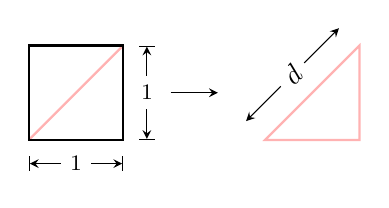
\begin{tikzpicture}[scale=1.2,>=stealth]
    \draw[thick,red!30] (0,0) -- (1,1);
    \draw[thick] (0,0) rectangle (1,1);
    \draw[|<->|] (0,-.25) -- node[fill=white,font=\footnotesize]{1} (1,-.25);
    \draw[|<->|] (1.25,0) -- node[fill=white,font=\footnotesize]{1} (1.25,1);

    \draw[->] (1.5,0.5) -- (2,0.5);

    \draw[thick,red!30] (2.5,0) -- (3.5,0) -- (3.5,1) -- cycle;
    \draw[<->] (2.3,.2) --node[sloped,fill=white]{\(d\)} ++(45:1.39);
  \end{tikzpicture}
  \caption{Representación de un cuadrado de lado uno y su diagonal}
  \label{fig:square}
\end{figure}

El teorema de Pitágoras, cuya justificación estudiaremos en geometría, permite relacionar los lados de un triángulo rectángulo. Aplicado al triángulo formado por dos lados del cuadrado y su diagonal \(d\), establece que
\[
d^2=1^2+1^2=2
\]

Por lo tanto, la diagonal debe ser un número positivo cuyo cuadrado sea \(2\).

Podemos preguntarnos entonces si alguna fracción representa exactamente esa longitud. Es decir, ¿existen enteros \(a\) y \(b\), con \(b\neq0\), tales que
\[
\left(\frac ab\right)^2=2?
\]

Supongamos que sí y que \(\frac ab\) está escrita en su forma irreducible. Entonces operamos sobre la expresión anterior, 
\begin{align*}
  \left(\frac ab\right)^2 &= 2 \\ 
  \frac{a^2}{b^2} &= 2 
\end{align*}
multiplicamos ambos miembros por \(b^2\):
\begin{align*}
  \frac{a^2}{b^2} b^2 &= 2b^2 \\
  \frac{b^2}{b^2} a^2 &= 2b^2 \\
  a^2&=2b^2
\end{align*}
Esto significa que \(a^2\) es par, ya que todo número multiplicado por \(2\) resulta ser un número par, y por lo tanto \(a\) también debe ser par. Podemos escribir \(a=2k\) para algún entero \(k\). Sustituyendo,
\[
(2k)^2=2b^2
\]
de donde
\[
4k^2=2b^2
\]
y, por tanto,
\[
b^2=2k^2
\]
Así, \(b^2\) también es par y, en consecuencia, \(b\) es par.

Pero entonces \(a\) y \(b\) tienen al menos un factor \(2\) en común, lo que contradice que \(\frac ab\) estuviera escrita en forma irreducible.

Por lo tanto, ningún número racional tiene cuadrado igual a \(2\).

Y aquí aparece algo importante. La diagonal del cuadrado no desaparece por el hecho de que ninguna fracción pueda representarla. Es una longitud perfectamente determinada por la figura; simplemente hemos descubierto que el conjunto \(\mathbb Q\) no contiene ningún número capaz de describirla exactamente.

Necesitamos entonces ampliar nuevamente nuestro sistema numérico.

Llamaremos \emph{números reales} a los números del conjunto \(\mathbb R\), que contiene a todos los racionales y también a números como el que representa la diagonal de este cuadrado. Este número se denota por
\[
\sqrt2.
\]
Por definición,
\[
\left(\sqrt2\right)^2=2,
\]
y acabamos de comprobar que
\[
\sqrt2\notin\mathbb Q.
\]

Los números reales que no son racionales reciben el nombre de \emph{irracionales}. Así,
\[
\sqrt2
\]
es un número irracional.

Una primera manera de imaginar \(\mathbb R\) es pensar en todos los números que pueden ubicarse sobre la recta numérica. Los racionales ocupan muchos de sus puntos, pero no todos. Los números irracionales permiten representar también aquellos puntos y longitudes que ninguna fracción puede describir exactamente.

De este modo,
\[
\mathbb N\subseteq\mathbb Z\subseteq\mathbb Q\subseteq\mathbb R.
\]

Construir rigurosamente el conjunto de los números reales requiere ideas que exceden nuestro propósito actual. Por ahora nos bastará una observación fundamental: una cantidad puede estar perfectamente determinada por un problema y, sin embargo, no pertenecer al conjunto numérico con el que veníamos trabajando. Cuando eso ocurre, necesitamos ampliar nuestro lenguaje numérico para poder representarla.

\begin{note}
Los números reales no son solamente objetos abstractos creados para hacer cálculos: aparecen de manera natural al describir numerosos fenómenos del mundo que nos rodea.

A medida que avance en el estudio de la matemática y la geometría encontrará algunos números especialmente importantes. Uno de ellos es
\[
\pi,
\]
llamado \emph{número pi} y representado mediante la letra griega pi minúscula. Aparece, por ejemplo, al estudiar circunferencias, áreas, ondas y movimientos periódicos.

Otro es
\[
e,
\]
conocido como \emph{número de Euler}. Surge de manera natural al estudiar procesos de crecimiento y decrecimiento continuo, como ciertos modelos de crecimiento poblacional, interés compuesto, fenómenos físicos y muchos otros procesos.

Estos números, junto con muchas de las ideas que irá aprendiendo, forman parte del lenguaje matemático utilizado para comprender la naturaleza y desarrollar gran parte de la ciencia y la tecnología modernas.
\end{note}

\subsection{Raíz \textit{n}-ésima}

Recapitulando lo que hemos visto; partimos de un número y de un exponente para calcular una potencia. Por ejemplo,
\[
2^3=8.
\]

Pero también podemos plantear el problema en sentido contrario:
\begin{center}
\textit{¿qué número elevado al cubo produce \(8\)?}
\end{center}
Como
\[
2^3=8,
\]
la respuesta es \(2\).

La radicación nace precisamente de esta pregunta. La expresión
\[
\sqrt[n]{a}
\]
se lee ``raíz \(n\)-ésima de \(a\)'' y busca un número que, elevado a \(n\), produzca \(a\).

En esta expresión, \(n\) recibe el nombre de \emph{índice} y \(a\) el de \emph{radicando}.

Por ejemplo,
\[
\sqrt[3]{8}=2
\]
porque
\[
2^3=8.
\]

Cuando el índice es \(2\), normalmente no se escribe:
\[
\sqrt a=\sqrt[2]{a}.
\]

Antes de definir con precisión qué valor representa una raíz, conviene observar algo que ya conocemos acerca de las potencias.

\subsection{¿Qué cambia si el índice es par o impar?}

Supongamos que queremos encontrar un número \(b\) que satisfaga
\[
b^n=a.
\]

Si \(b\) es positivo, su potencia será positiva cualquiera sea \(n\). La diferencia aparece cuando \(b\) es negativo.

Ya vimos que una cantidad par de factores negativos produce un resultado positivo, mientras que una cantidad impar produce un resultado negativo. Por ello,
\[
(-b)^n=
\begin{cases}
b^n, & \text{si \(n\) es par},\\
-b^n, & \text{si \(n\) es impar}.
\end{cases}
\]

Esta diferencia es la que determina el comportamiento de las raíces.

\subsubsection{Cuando el índice es impar}

Consideremos primero un índice impar, por ejemplo \(3\).

Tenemos
\[
2^3=8
\]
y también
\[
(-2)^3=-8.
\]

Al elevar a un exponente impar, el signo se conserva:
\[
\text{positivo}^{\text{impar}}=\text{positivo},
\qquad
\text{negativo}^{\text{impar}}=\text{negativo}.
\]

Por eso podemos buscar raíces impares tanto de números positivos como de números negativos:
\[
\sqrt[3]{8}=2,
\qquad
\sqrt[3]{-8}=-2.
\]

Además, elevar a una potencia impar no hace que un número y su opuesto produzcan el mismo resultado:
\[
2^3=8,
\qquad
(-2)^3=-8.
\]

De hecho, si aumentamos el número que usamos como base, también aumenta su potencia impar. Por ejemplo,
\[
1^3<2^3<3^3,
\]
y
\[
(-3)^3<(-2)^3<(-1)^3.
\]

Este comportamiento permite que cada número real tenga una única raíz real cuando el índice es impar.

Por lo tanto, si \(n\) es impar,
\[
\sqrt[n]{a}=b
\quad\Longleftrightarrow\quad
b^n=a.
\]

Por ejemplo,
\[
\sqrt[5]{32}=2
\]
porque
\[
2^5=32,
\]
mientras que
\[
\sqrt[5]{-32}=-2
\]
porque
\[
(-2)^5=-32.
\]

\subsubsection{Cuando el índice es par}

Veamos ahora qué ocurre con un índice par, por ejemplo \(2\).

Tenemos
\[
5^2=25,
\]
pero también
\[
(-5)^2=25.
\]

Esto sucede porque
\[
(-5)^2=(-5)(-5)=25.
\]

Lo mismo ocurre con cualquier exponente par: los factores negativos pueden agruparse de dos en dos y el resultado es no negativo.

Por ejemplo,
\[
(-2)^4=16,
\qquad
(-3)^6=729.
\]

Por lo tanto, ninguna potencia real de exponente par puede producir un número negativo.

Esto explica por qué una expresión como
\[
\sqrt{-4}
\]
no representa un número real: no existe ningún número real \(b\) que satisfaga
\[
b^2=-4.
\]

Si probamos con un número positivo,
\[
b^2>0,
\]
y si probamos con uno negativo, su cuadrado también es positivo. Finalmente,
\[
0^2=0.
\]
Ninguna de las posibilidades produce \(-4\).

En cambio, para un radicando positivo aparece otra cuestión.

Sabemos que
\[
5^2=25
\]
y
\[
(-5)^2=25.
\]

Por lo tanto, la ecuación
\[
b^2=25
\]
tiene dos soluciones reales:
\[
b=5
\qquad\text{y}\qquad
b=-5.
\]

Entonces podríamos preguntarnos:

\[
\text{¿qué valor debe representar \(\sqrt{25}\)?}
\]

Para que el símbolo radical represente una sola cantidad y no dos valores diferentes, se adopta la convención de elegir la solución no negativa.

Así,
\[
\sqrt{25}=5,
\]
y no \(\pm5\).

El número elegido recibe el nombre de \emph{raíz principal}.

En general, si \(n\) es par y \(a\ge0\),
\[
\sqrt[n]{a}=b
\]
significa que
\[
b^n=a
\qquad\text{y}\qquad
b\ge0.
\]

Por lo tanto,
\[
\sqrt[4]{16}=2,
\]
aunque también sea cierto que
\[
(-2)^4=16.
\]

La expresión
\[
\sqrt[4]{16}
\]
representa solamente la raíz principal, es decir, \(2\).

\begin{note}
Hay una diferencia importante entre
\[
\sqrt{25}=5
\]
y resolver la ecuación
\[
x^2=25.
\]

El radical \(\sqrt{25}\) representa, por definición, una sola cantidad: la raíz principal no negativa.

En cambio, al resolver
\[
x^2=25,
\]
debemos buscar todos los números cuyo cuadrado sea \(25\). Por eso las soluciones son
\[
x=5
\qquad\text{y}\qquad
x=-5.
\]
\end{note}

La existencia de raíces \(n\)-ésimas para todos los números reales permitidos puede demostrarse rigurosamente a partir de propiedades más profundas de los números reales. Por ahora nos concentraremos en comprender cómo se comportan y cómo operar con ellas.

\subsection{El radical representa un solo número}

Es importante distinguir una raíz de las soluciones de una ecuación.

Por ejemplo,
\[
\sqrt{25}=5.
\]

El símbolo \(\sqrt{\phantom a}\) representa una sola cantidad. Como se trata de una raíz de índice par, elegimos por definición la raíz no negativa.

Sin embargo, si preguntamos
\[
\text{¿qué números elevados al cuadrado producen \(25\)?}
\]
encontramos dos respuestas:
\[
5^2=25
\]
y
\[
(-5)^2=25.
\]

Por lo tanto, la ecuación
\[
x^2=25
\]
tiene dos soluciones:
\[
x=5
\qquad\text{o}\qquad
x=-5.
\]

Podemos escribirlas de manera abreviada como
\[
x=\pm5.
\]

El signo \(\pm\) no forma parte del valor de
\[
\sqrt{25}.
\]
Aparece porque estamos reuniendo las dos soluciones posibles de la ecuación.

Así,
\[
\boxed{\sqrt{25}=5}
\]
pero
\[
\boxed{x^2=25\quad\Longrightarrow\quad x=\pm5}.
\]

Hay una razón por la que debemos tener este cuidado. Al elevar un número a un exponente par, su signo puede dejar de distinguirse:
\[
3^2=9
\qquad\text{y}\qquad
(-3)^2=9.
\]

Una vez obtenido el \(9\), ya no podemos saber solamente a partir de ese resultado si el número original era \(3\) o \(-3\).

Por ahora evitaremos utilizar la raíz como una operación mecánica para ``deshacer'' potencias dentro de ecuaciones. Más adelante estudiaremos herramientas que nos permitirán hacerlo de manera segura.

En cambio, cuando simplemente calculamos una expresión como
\[
\sqrt{36},
\]
no existe ambigüedad:
\[
\sqrt{36}=6.
\]

El radical representa siempre el valor principal que hemos definido.


\subsection{Algoritmo para aproximar raíces}

Algunas raíces pueden reconocerse inmediatamente:
\[
\sqrt{25}=5
\]
porque
\[
5^2=25,
\]
o
\[
\sqrt[3]{125}=5
\]
porque
\[
5^3=125.
\]

Pero no siempre ocurre esto.

Consideremos, por ejemplo,
\[
\sqrt{17}.
\]

Estamos buscando un número cuyo cuadrado sea \(17\). No parece haber un número entero que lo produzca exactamente, pero podemos comenzar buscando entre qué números se encuentra.

Sabemos que
\[
4^2=16
\]
y
\[
5^2=25.
\]

Como
\[
16<17<25,
\]
la raíz debe encontrarse entre \(4\) y \(5\):
\[
4<\sqrt{17}<5.
\]

Ahora podemos investigar los décimos.

Probemos con \(4{,}1\):
\[
4{,}1^2=16{,}81.
\]

Todavía estamos por debajo de \(17\).

Probemos con \(4{,}2\):
\[
4{,}2^2=17{,}64.
\]

Ahora nos hemos pasado. Por lo tanto,
\[
4{,}1<\sqrt{17}<4{,}2.
\]

Podemos continuar de la misma manera con los centésimos:
\[
4{,}12^2=16{,}9744,
\]
mientras que
\[
4{,}13^2=17{,}0569.
\]

Entonces,
\[
4{,}12<\sqrt{17}<4{,}13.
\]

Si necesitamos mayor precisión, podemos repetir nuevamente el procedimiento:
\[
4{,}123^2=16{,}999129,
\]
mientras que
\[
4{,}124^2=17{,}007376.
\]

Así,
\[
4{,}123<\sqrt{17}<4{,}124.
\]

Podemos continuar tanto como sea necesario.

Este procedimiento nos proporciona aproximaciones cada vez mejores:
\[
\sqrt{17}\approx4{,}123.
\]

Observe que
\[
\sqrt{17}
\]
y
\[
4{,}123
\]
no significan exactamente lo mismo. El radical representa el número exacto; el decimal es solamente una aproximación.

\subsubsection{Un procedimiento general}

Para aproximar una raíz \(n\)-ésima podemos proceder de la siguiente manera:

\begin{enumerate}
    \item Buscamos dos números entre cuyas potencias \(n\)-ésimas se encuentre el radicando.
    \item Con ello sabemos entre qué dos números se encuentra la raíz.
    \item Probamos valores intermedios para estrechar el intervalo.
    \item Repetimos el procedimiento hasta alcanzar la precisión que necesitemos.
\end{enumerate}

Por ejemplo, para aproximar
\[
\sqrt[3]{390},
\]
comenzamos observando que
\[
7^3=343
\]
y
\[
8^3=512.
\]

Como
\[
343<390<512,
\]
sabemos que
\[
7<\sqrt[3]{390}<8.
\]

Probemos ahora con décimos:
\[
7{,}3^3=389{,}017,
\]
mientras que
\[
7{,}4^3=405{,}224.
\]

Por tanto,
\[
7{,}3<\sqrt[3]{390}<7{,}4.
\]

Podemos seguir probando centésimos y milésimos si necesitamos una aproximación más precisa.

No todas las raíces producen un número sencillo que podamos reconocer de inmediato. En esos casos, conservar el radical,
\[
\sqrt{17},
\]
nos permite representar el valor de manera exacta, mientras que una escritura como
\[
4{,}123
\]
nos proporciona una aproximación útil.

\begin{note}
Es normal sentir que expresiones como
\[
\sqrt{17}
\qquad\text{o}\qquad
\sqrt[3]{390}
\]
son cálculos que todavía deben ``resolverse''. Sin embargo, el radical ya representa un número.

Cuando una raíz puede reconocerse exactamente, escribimos su valor:
\[
\sqrt{25}=5.
\]
Pero si no existe un valor sencillo que podamos reconocer, no es necesario reemplazar la raíz por una aproximación decimal. En matemáticas suele preferirse conservar la expresión exacta:
\[
\sqrt{17}.
\]

Una escritura decimal como
\[
\sqrt{17}\approx4{,}1231
\]
es solamente una aproximación y se utiliza cuando el problema requiere conocer un valor numérico aproximado.

Actualmente, calculadoras y computadoras pueden obtener aproximaciones con una precisión enorme utilizando algoritmos numéricos que refinan progresivamente el resultado. El procedimiento de acotar la raíz que hemos visto comparte esa misma idea general: comenzar con información aproximada e ir acercándose cada vez más al valor buscado.

Por ahora, lo más importante es recordar que
\[
\boxed{\sqrt{17}\text{ ya es un número}}
\]
y constituye una respuesta exacta. No necesita transformarlo en un decimal a menos que el problema lo solicite o que una aproximación resulte útil para el cálculo que está realizando.
\end{note}


\section{Potencias con exponentes racionales}

Hasta ahora hemos dado significado a expresiones como
\[
a^3,\qquad a^0,\qquad a^{-2},
\]
es decir, a potencias cuyos exponentes son números enteros.

Queremos ahora comprender qué podría significar que el exponente sea una fracción:
\[
a^{1/2},
\qquad
a^{1/3},
\qquad
a^{2/5}.
\]

La idea será la misma que hemos seguido hasta ahora: no inventaremos una regla nueva de manera aislada, sino que buscaremos una definición compatible con las propiedades de las potencias que ya conocemos.

Para evitar dificultades relacionadas con los signos, comenzaremos trabajando con
\[
a>0.
\]

\subsection{El significado de exponentes fraccionarios}

Comencemos con un exponente sencillo:
\[
a^{1/2}.
\]

Sabemos que una potencia de otra potencia satisface
\[
(a^m)^n=a^{mn}.
\]

Si queremos que esta propiedad siga siendo válida al introducir exponentes fraccionarios, entonces debería ocurrir que
\[
\left(a^{1/2}\right)^2
=
a^{(1/2)\cdot2}
=
a^1
=
a.
\]

Por lo tanto, \(a^{1/2}\) debe representar un número cuyo cuadrado sea \(a\).

Pero ya tenemos una operación que responde exactamente a esa pregunta:
\[
\sqrt a.
\]

Por eso definimos
\[
a^{1/2}=\sqrt a.
\]

El mismo razonamiento puede hacerse con cualquier entero positivo \(q\). Si queremos que
\[
\left(a^{1/q}\right)^q
=
a^{(1/q)q}
=
a,
\]
entonces \(a^{1/q}\) debe ser el número cuya potencia \(q\)-ésima es \(a\).

Por lo tanto,
\[
\boxed{a^{1/q}=\sqrt[q]{a}}.
\]

Así, por ejemplo,
\[
16^{1/2}=\sqrt{16}=4
\]
y
\[
8^{1/3}=\sqrt[3]{8}=2.
\]

El exponente fraccionario \(1/q\) no introduce entonces una operación completamente nueva: es otra manera de escribir una raíz.

\subsubsection{Exponentes fraccionarios de la forma \(p/q\)}

Consideremos ahora un exponente como
\[
\frac{p}{q},
\]
donde inicialmente supondremos que \(p\) y \(q\) son naturales positivos.

Podemos escribir
\[
\frac pq=p\cdot\frac1q.
\]

Utilizando nuevamente la propiedad de una potencia elevada a otra potencia,
\[
a^{p/q}
=
a^{p(1/q)}
=
\left(a^{1/q}\right)^p.
\]

Como acabamos de establecer que
\[
a^{1/q}=\sqrt[q]{a},
\]
obtenemos
\[
\boxed{
a^{p/q}
=
\left(\sqrt[q]{a}\right)^p
}.
\]

Esto nos da una forma concreta de interpretar el exponente racional:

\begin{enumerate}
    \item calculamos la raíz \(q\)-ésima de la base;
    \item elevamos el resultado a la potencia \(p\).
\end{enumerate}

Por ejemplo,
\[
8^{2/3}
=
\left(\sqrt[3]{8}\right)^2
=
2^2
=
4.
\]

\subsection{¿Podemos realizar las operaciones en el orden contrario?}

Ya vimos que
\[
a^{p/q}
=
\left(\sqrt[q]{a}\right)^p.
\]

Esto significa que podemos calcular primero la raíz \(q\)-ésima y después elevar el resultado a la potencia \(p\).

Pero observemos nuevamente el exponente:
\[
\frac pq
=
p\cdot\frac1q.
\]

Como la multiplicación es conmutativa, también podemos escribir
\[
\frac pq
=
\frac1q\cdot p.
\]

Los dos factores son exactamente los mismos. Solo hemos cambiado su orden.

Y aquí ocurre algo interesante.

Si una potencia elevada a otra potencia multiplica sus exponentes, entonces
\[
a^{p/q}
=
a^{(1/q)p}
=
\left(a^p\right)^{1/q}.
\]

Pero ya sabemos que un exponente de la forma \(1/q\) representa una raíz \(q\)-ésima:
\[
x^{1/q}=\sqrt[q]{x}.
\]

Por lo tanto,
\[
\left(a^p\right)^{1/q}
=
\sqrt[q]{a^p}.
\]

Así obtenemos
\[
\boxed{
a^{p/q}
=
\left(\sqrt[q]{a}\right)^p
=
\sqrt[q]{a^p}
}.
\]

Podemos verlo directamente en los exponentes:
\[
p\cdot\frac1q
=
\frac1q\cdot p.
\]

En el primer orden,
\[
\left(a^{1/q}\right)^p,
\]
calculamos primero la raíz y después la potencia.

En el segundo,
\[
\left(a^p\right)^{1/q},
\]
calculamos primero la potencia y después la raíz.

No son dos reglas diferentes. Son las mismas operaciones realizadas en distinto orden.

Veamos un ejemplo:
\[
27^{2/3}.
\]

Podemos calcular primero la raíz:
\[
27^{2/3}
=
\left(\sqrt[3]{27}\right)^2
=
3^2
=
9.
\]

O podemos calcular primero la potencia:
\[
27^{2/3}
=
\sqrt[3]{27^2}
=
\sqrt[3]{729}
=
9.
\]

En ambos casos llegamos al mismo resultado.

Normalmente convendrá elegir el camino que produzca cálculos más sencillos. En este ejemplo,
\[
\sqrt[3]{27}=3
\]
hace que calcular primero la raíz sea mucho más cómodo que comenzar con
\[
27^2=729.
\]

\subsection{La fracción utilizada no puede cambiar el resultado}

Hay todavía un detalle importante.

Sabemos que una misma fracción puede escribirse de muchas maneras:
\[
\frac12=\frac24=\frac36=\cdots
\]

Por lo tanto, si utilizamos estas fracciones como exponentes, todas deben producir el mismo resultado.

Por ejemplo,
\[
16^{1/2}=4.
\]

Pero también podemos escribir
\[
\frac12=\frac24.
\]

Entonces deberíamos obtener igualmente
\[
16^{2/4}=4.
\]

Y, en efecto,
\[
16^{2/4}
=
\sqrt[4]{16^2}
=
\sqrt[4]{256}
=
4.
\]

No parece haber ningún problema.

Pero queremos asegurarnos de que esto ocurra siempre.

Supongamos que tenemos el exponente
\[
\frac pq
\]
y multiplicamos su numerador y su denominador por el mismo número natural positivo \(k\):
\[
\frac pq=\frac{pk}{qk}.
\]

Utilizando la primera fracción obtenemos
\[
a^{p/q}
=
\sqrt[q]{a^p}.
\]

Ahora preguntémonos: ¿qué sucede si usamos la segunda?
Obtendríamos
\[
a^{pk/qk}
=
\sqrt[qk]{a^{pk}}.
\]

A primera vista las dos raíces parecen bastante diferentes:
\[
\sqrt[q]{a^p}
\qquad\text{y}\qquad
\sqrt[qk]{a^{pk}}.
\]

Para comprobar si son iguales, planteamos la igualdad:
\begin{align*}
  \sqrt[q]{a^p} &\stackrel{?}{=} \sqrt[qk]{a^{pk}} \\ 
  \left(\sqrt[q]{a^p}\right)^{qk}
  &\stackrel{?}{=}
  \left(\sqrt[qk]{a^{pk}}\right)^{qk}
\end{align*}

Aplicando las propiedades de los exponentes y las raíces que hemos visto:
\begin{align*}
  \left(\sqrt[q]{a^p}\right)^{qk}
  &\stackrel{?}{=}
  \left(a^{pk}\right)^{\frac{qk}{qk}} \\ 
  \left(a^p\right)^{\frac{qk}{q}}
  &\stackrel{?}{=}
  a^{pk} \\ 
  \left(a^p\right)^k
  &\stackrel{?}{=}
  a^{pk} \\ 
  a^{pk}
  &\stackrel{?}{=}
  a^{pk}.
\end{align*}

La última igualdad es verdadera. Además, como estamos trabajando con raíces principales, las dos expresiones originales son positivas. Por lo tanto, si sus potencias \(qk\)-ésimas son iguales, ellas también deben ser iguales.

Así,
\[
\sqrt[q]{a^p}
=
\sqrt[qk]{a^{pk}}.
\]

Y, en consecuencia,
\[
\boxed{
a^{p/q}=a^{pk/qk}
}.
\]

Así que ampliar una fracción no cambia el valor de la potencia.

Por ejemplo,
\[
\frac12=\frac24,
\]
y por eso
\[
16^{1/2}
=
16^{2/4}
=
4.
\]

Lo mismo ocurriría con
\[
\frac12=\frac36,
\qquad
\frac23=\frac46,
\qquad
\frac34=\frac68,
\]
o con cualquier otra fracción equivalente.

Esto es fundamental: el valor de
\[
a^{p/q}
\]
depende del número racional \(\frac pq\), no de la manera particular en que hayamos escrito esa fracción.

\subsection{Numerador cero o negativo}

Hasta ahora supusimos que \(p>0\). Podemos completar la definición utilizando lo que ya sabemos sobre exponentes enteros.

Si
\[
p=0,
\]
entonces
\[
\frac pq=0,
\]
y recuperamos
\[
a^{0/q}=a^0=1.
\]

Si \(p<0\), utilizamos la misma idea que empleamos para los exponentes enteros negativos: el exponente negativo indica el inverso multiplicativo.

Así,
\[
a^{-p/q}
=
\frac{1}{a^{p/q}}.
\]

Por ejemplo,
\[
8^{-2/3}
=
\frac{1}{8^{2/3}}.
\]

Como
\[
8^{2/3}
=
\left(\sqrt[3]{8}\right)^2
=
2^2
=
4,
\]
obtenemos
\[
8^{-2/3}
=
\frac14.
\]

De este modo, para una base positiva \(a\), los exponentes racionales quedan conectados con operaciones que ya conocemos: potencias, raíces e inversos multiplicativos.

\subsection{Base cero}

Para \(r\in\mathbb Q\) positivo, podemos definir
\[
0^r=0.
\]
Pero \(0^0\) queda sin definir en este capítulo y \(0^r\) tampoco está definido cuando \(r<0\), porque un exponente negativo exigiría dividir por una potencia de cero.

\subsection{Bases negativas}

Hasta ahora hemos trabajado principalmente con bases positivas. Con ellas, las raíces y los exponentes racionales se comportan de una manera bastante cómoda.

Con las bases negativas debemos prestar un poco más de atención.

Comencemos con algo que ya conocemos:
\[
(-8)^{1/3}.
\]

Como el exponente \(1/3\) indica una raíz cúbica,
\[
(-8)^{1/3}
=
\sqrt[3]{-8}
=
-2.
\]

No hay ningún problema: una cantidad negativa puede tener una raíz de índice impar, ya que
\[
(-2)^3=-8.
\]

Algo parecido ocurre con
\[
(-8)^{2/3}.
\]

Primero calculamos la raíz cúbica y después elevamos al cuadrado:
\[
(-8)^{2/3}
=
\left(\sqrt[3]{-8}\right)^2
=
(-2)^2
=
4.
\]

Observemos algo interesante: la base sigue siendo negativa, pero ahora el resultado es positivo.

Esto no es extraño. La raíz cúbica nos dio \(-2\), y al elevarlo al cuadrado desapareció el signo negativo.

En general, si escribimos el exponente racional en su forma irreducible
\[
\frac pq,
\]
el denominador \(q\) nos indica qué raíz debemos calcular.

Si \(q\) es impar, podemos calcular una raíz \(q\)-ésima de un número negativo dentro de los números reales.

Por ejemplo,
\[
\sqrt[3]{-8}=-2,
\qquad
\sqrt[5]{-32}=-2.
\]

Después, el numerador \(p\) nos indica a qué potencia debemos elevar ese resultado. Según sea esa potencia par o impar, el signo final puede cambiar.

Pero si \(q\) es par, aparece un problema.

Por ejemplo,
\[
(-16)^{1/4}
=
\sqrt[4]{-16}.
\]

No existe ningún número real cuya cuarta potencia sea \(-16\), porque una potencia par de un número real nunca es negativa.

Por lo tanto,
\[
(-16)^{1/4}
\]
no representa un número real.

\subsubsection*{Una pequeña trampa}

Aquí aparece una razón muy importante para reducir siempre la fracción del exponente.

Sabemos que
\[
\frac13=\frac26.
\]

Por lo tanto,
\[
(-8)^{1/3}
\qquad\text{y}\qquad
(-8)^{2/6}
\]
tienen exactamente el mismo exponente.

Ya sabemos que
\[
(-8)^{1/3}=-2.
\]

Pero imaginemos que tomamos \(2/6\) sin reducirlo y aplicamos mecánicamente la expresión
\[
a^{p/q}=\sqrt[q]{a^p}.
\]

Obtendríamos
\[
(-8)^{2/6}
\stackrel{?}{=}
\sqrt[6]{(-8)^2}
=
\sqrt[6]{64}
=
2.
\]

¡Pero acabamos de obtener \(2\) cuando antes habíamos obtenido \(-2\)!

El problema no está en que
\[
\frac13
\quad\text{y}\quad
\frac26
\]
sean exponentes diferentes. Son exactamente el mismo número racional.

El problema es que, al utilizar \(2/6\) sin reducir, introdujimos artificialmente una raíz de índice par. Al elevar primero \(-8\) al cuadrado, además, perdimos el signo negativo antes de calcular la raíz.

Por eso, cuando la base es negativa, primero debemos escribir el exponente racional en su forma irreducible:
\[
\frac26=\frac13.
\]

Entonces calculamos
\[
(-8)^{2/6}
=
(-8)^{1/3}
=
\sqrt[3]{-8}
=
-2.
\]

Así evitamos que una forma innecesariamente complicada de escribir la fracción nos lleve por un camino equivocado.

Podemos encontrar una situación todavía más peligrosa.

Consideremos
\[
(-5)^{2/4}.
\]

Si observamos solamente la expresión tal como está escrita, podríamos pensar en calcular primero la potencia:
\[
(-5)^{2/4}
\stackrel{?}{=}
\sqrt[4]{(-5)^2}.
\]

Entonces,
\[
\sqrt[4]{(-5)^2}
=
\sqrt[4]{25}
=
\sqrt{5}.
\]

¡Parece que hemos encontrado un resultado perfectamente válido! Pero algo huele mal de este resultado. Observemos que ocurre si intentamos verificar la solución. 

Supuestamente decimos que 
\[
  (-5)^{2/4} = \sqrt5
\]
En otras palabras, aplicando la definición de raíz:
\[
  (-5)^2 = \left(\sqrt{5}\right)^4
\]
Es decir, 
\[
  (-5)^2 = (5)^2
\]
Lo cual es verdad. Sin embargo observemos un detalle sutil: los números de la base no son iguales, a pesar de que el resultado final si lo es.

Pero hagamos algo que siempre debemos hacer con un exponente racional: reduzcamos primero la fracción.

Como
\[
\frac24=\frac12,
\]
la expresión original es en realidad
\[
(-5)^{1/2}.
\]

Y eso significa
\[
\sqrt{-5},
\]
que no es un número real.

Así que hemos llegado a una situación bastante grave. Por un camino logramos encontrar que:
\[
(-5)^{2/4}
\stackrel{?}{=}
\sqrt5
\]
mientras que por otro camino llegamos a:
\[
(-5)^{2/4}
=
(-5)^{1/2}
\]
que nos muestra que la expresión no representa ningún número real.

¿Qué ocurrió?

Al elevar primero \(-5\) al cuadrado obtuvimos
\[
(-5)^2=25.
\]

En ese instante desapareció el signo negativo. Después calculamos una raíz cuarta de un número positivo y todo pareció funcionar.

Pero habíamos ocultado el verdadero problema.

El exponente
\[
\frac24
\]
no es un número racional diferente de
\[
\frac12.
\]

Son exactamente el mismo número:
\[
\frac24=\frac12.
\]

Por lo tanto, no podemos permitir que una forma distinta de escribir el mismo exponente cambie si la potencia existe o incluso produzca un resultado diferente.

Este ejemplo nos muestra por qué, con bases negativas, reducir primero el exponente racional no es solamente una comodidad:
\[
\boxed{\text{es necesario para interpretar correctamente la potencia.}}
\]

Así, ante una expresión como
\[
(-5)^{2/4},
\]
primero escribimos
\[
\frac24=\frac12.
\]

Entonces vemos inmediatamente que
\[
(-5)^{2/4}
=
(-5)^{1/2}
\]
no representa un número real.

El valor \(\sqrt5\) que apareció antes no era una segunda respuesta posible. Fue el resultado de seguir un camino algebraico que, en este caso, no era válido.

Podemos resumir la idea de esta manera:

Si la base es negativa, primero reducimos el exponente
\[
\frac pq
\]
a su forma irreducible.

Luego observamos su denominador:
\[
\boxed{
\begin{array}{c}
q\text{ impar} \quad\longrightarrow\quad
\text{la potencia puede representar un número real},\\[4pt]
q\text{ par} \quad\longrightarrow\quad
\text{la potencia no representa un número real}.
\end{array}
}
\]
Por esta razón, cuando estudiemos las propiedades generales de los exponentes racionales utilizaremos normalmente bases positivas. Así podremos concentrarnos en las propiedades mismas sin detenernos constantemente a comprobar qué raíces existen en los números reales.


\section{Propiedades generales}

Las extensiones realizadas no fueron elecciones independientes. Definimos los exponentes cero, negativos y racionales para conservar, siempre que fuera posible, las relaciones descubiertas al contar factores. Podemos ahora reunirlas en un mismo marco.

Sean \(a,b>0\) y \(r,s\in\mathbb Q\). Entonces:
\begin{gather*}
a^r\cdot a^s=a^{r+s},\\
\frac{a^r}{a^s}=a^{r-s},\\
(a^r)^s=a^{r\cdot s},\\
(a\cdot b)^r=a^r\cdot b^r,\\
\left(\frac ab\right)^r=\frac{a^r}{b^r}.
\end{gather*}

La primera propiedad reúne cantidades de factores de una misma base; la segunda expresa la cancelación mediante una resta; la tercera cuenta cuántas veces se repite una repetición; las dos últimas distribuyen una misma potencia entre los factores de un producto o de un cociente.

\begin{example}[Simplificar sin aproximar]
Considere
\[
2^{3/4}\cdot2^{5/4}.
\]
Como las bases son iguales y positivas,
\[
2^{3/4}\cdot2^{5/4}
=
2^{3/4+5/4}
=
2^{8/4}
=
2^2
=
4.
\]
No fue necesario obtener aproximaciones decimales de cada factor.
\end{example}

\begin{example}[Un exponente negativo]
La expresión
\[
\frac{3^{1/2}}{3^{5/2}}
\]
puede simplificarse como
\[
3^{1/2-5/2}=3^{-2}=\frac1{3^2}=\frac19.
\]
Cada paso conserva el número representado y hace visible una relación diferente.
\end{example}

\subsection{Las condiciones forman parte de la propiedad}

Las propiedades que hemos estudiado son herramientas muy poderosas, pero no podemos utilizarlas sin mirar las condiciones bajo las cuales son válidas.

Esto es especialmente importante cuando aparecen divisiones, raíces o bases negativas.

Por ejemplo, consideremos
\[
\left((-8)^{2/3}\right)^{3/2}.
\]

Podemos calcular la expresión tal como está escrita, comenzando por la potencia interior:
\[
(-8)^{2/3}
=
\left(\sqrt[3]{-8}\right)^2
=
(-2)^2
=
4.
\]

Ahora calculamos la potencia exterior:
\[
4^{3/2}
=
\left(\sqrt{4}\right)^3
=
2^3
=
8.
\]

Por lo tanto,
\[
\boxed{
\left((-8)^{2/3}\right)^{3/2}=8
}.
\]

Pero aquí aparece una tentación.

Conocemos la propiedad
\[
(a^r)^s=a^{rs},
\]
así que podríamos intentar escribir
\[
\left((-8)^{2/3}\right)^{3/2}
\stackrel{?}{=}
(-8)^{(2/3)(3/2)}
=
(-8)^1
=
-8.
\]

Ahora tenemos
\[
8\neq -8.
\]

¿Significa esto que la expresión puede tener dos resultados?

No.

La expresión original tiene un único resultado:
\[
8.
\]

Lo que falló fue nuestra transformación.

La propiedad
\[
(a^r)^s=a^{rs}
\]
no puede utilizarse sin cuidado cuando la base es negativa y aparecen exponentes racionales. En este libro la enunciaremos para
\[
a>0,
\]
precisamente para evitar estas situaciones.

Como en nuestro ejemplo la base original es
\[
-8<0,
\]
no teníamos permiso para multiplicar directamente los exponentes.

Cuando una propiedad no puede aplicarse, simplemente conservamos la expresión original y realizamos las operaciones en el orden indicado:
\[
\left((-8)^{2/3}\right)^{3/2}.
\]

Primero:
\[
(-8)^{2/3}=4.
\]

Después:
\[
4^{3/2}=8.
\]

Este ejemplo nos deja una regla práctica importante:
\begin{center}
  \textit{Antes de aplicar una propiedad, debemos comprobar que sus condiciones se cumplen.}
\end{center}

Si las condiciones no se cumplen, eso no significa necesariamente que la expresión original esté mal definida. Significa solamente que esa propiedad no puede utilizarse para transformarla.

Lo mismo ocurre con otras propiedades.

Por ejemplo, en
\[
\frac{a^r}{a^s},
\]
debemos exigir
\[
a\neq0,
\]
porque estamos dividiendo entre \(a^s\).

Y con exponentes racionales debemos vigilar las bases negativas, porque algunas raíces no existen dentro de los números reales.

Por eso las condiciones no son pequeños avisos añadidos después de aprender una propiedad. Forman parte de ella.

Si recordamos una propiedad, por ejemplo:
\[
(a^r)^s=a^{rs}.
\]
debemos tener presente sus restricciones. Que surgen directamente de no poder generalizar su comportamiento en ciertos rangos de valores.

\begin{note}
No piense en las propiedades matemáticas como reglas que hay que memorizar junto con una lista de restricciones.

Una propiedad aparece cuando descubrimos que cierto comportamiento se cumple de manera general.

Por ejemplo, puede ocurrir que una igualdad sea válida para todos los números positivos. En ese caso hemos encontrado una propiedad, pero su alcance llega solamente hasta allí: no tenemos derecho a suponer que también funciona con números negativos, con cero o con cualquier otro número fuera de las condiciones bajo las cuales fue demostrada.

Las restricciones simplemente nos indican hasta dónde llega la generalización.

Por eso, ante la duda, una buena estrategia es intentar reconstruir la propiedad.

Pregúntese:
\[
\text{¿por qué debería cumplirse esta igualdad?}
\]

Si puede demostrarla de manera general para los números que está utilizando, entonces puede aplicarla con seguridad. Si la demostración solamente funciona bajo ciertas condiciones, esas condiciones forman parte de la propiedad.

Así, en lugar de memorizar
\[
\text{propiedad}+\text{restricciones},
\]
intente comprender de dónde surge la propiedad.

Las restricciones no son excepciones molestas que debemos recordar después. Son precisamente las fronteras que nos indican dónde nuestro razonamiento sigue siendo válido.
\end{note}

En los enunciados generales de este capítulo utilizaremos normalmente bases positivas. Esto nos permitirá aplicar las propiedades con seguridad y concentrarnos en las ideas que queremos estudiar.

\subsection{Radicales y potencias}

Para \(a\ge0\) y \(n>1\),
\[
\sqrt[n]{a}=a^{1/n}.
\]
Esta equivalencia permite pasar de una escritura radical a una potencia racional y viceversa. Por ejemplo,
\[
\sqrt[5]{x^3}=x^{3/5}
\]
si \(x>0\).

También permite comprender propiedades de los radicales a partir de las potencias. Si \(a,b\ge0\),
\[
\sqrt[n]{a\cdot b}
=(a\cdot b)^{1/n}
=a^{1/n}b^{1/n}
=\sqrt[n]{a}\cdot\sqrt[n]{b}.
\]
Cuando el índice es par, las condiciones \(a,b\ge0\) garantizan que todas las raíces sean reales. Para índices impares pueden admitirse radicandos negativos, pero deben revisarse las condiciones de cada expresión.

No existe, en cambio, una distribución de la raíz sobre la suma:
\[
\sqrt{a+b}\ne\sqrt a+\sqrt b
\]
en general. Por ejemplo,
\[
\sqrt{9+16}=5,
\qquad
\sqrt9+\sqrt{16}=3+4=7.
\]


\section{Práctica con potencias y raíces}

En los siguientes ejercicios conviene indicar las propiedades utilizadas y comprobar que cada expresión esté definida antes de transformarla. Evaluar no siempre significa obtener un decimal: una potencia o un radical puede ser la representación exacta más clara del número.

\subsection*{Traducir productos y potencias}

Reescriba cada producto como una potencia. Luego evalúe cuando resulte sencillo.

\begin{enumerate}
\item \(2\cdot2\cdot2\cdot2\cdot2\)
\item \(7\cdot7\cdot7\)
\item \((-3)\cdot(-3)\cdot(-3)\cdot(-3)\)
\item \(\dfrac25\cdot\dfrac25\cdot\dfrac25\)
\item \(10\cdot10\cdot10\cdot10\cdot10\cdot10\)
\end{enumerate}

Ahora reescriba cada potencia como un producto de factores iguales.

\begin{enumerate}
\item \(4^3\)
\item \(3^5\)
\item \((-2)^4\)
\item \(\left(\dfrac12\right)^3\)
\item \(a^6\)
\end{enumerate}

\subsection*{Base, exponente y valor}

En cada expresión indique la base y el exponente. Luego encuentre su valor.

\begin{enumerate}
\item \(2^6\)
\item \(5^3\)
\item \((-4)^2\)
\item \(-4^2\)
\item \((-1)^9\)
\item \(9^1\)
\item \(12^0\)
\item \(0^5\)
\end{enumerate}

Explique por qué no se pide evaluar \(0^0\) junto con los ejemplos anteriores.

\subsection*{Aplicar propiedades con exponentes naturales}

Reescriba cada expresión como una sola potencia cuando sea posible y luego evalúe.

\begin{enumerate}
\item \(2^3\cdot2^5\)
\item \(7^2\cdot7^4\)
\item \(\dfrac{5^7}{5^3}\)
\item \(\dfrac{3^6}{3^6}\)
\item \((2^3)^4\)
\item \((5^2)^3\)
\item \(2^4\cdot3^4\)
\item \(\left(\dfrac23\right)^3\)
\end{enumerate}

Indique por qué no puede aplicarse la regla de igual base a \(2^3\cdot3^4\).

\subsection*{Reconocer igualdades falsas}

Decida si cada igualdad es verdadera para todos los valores en que aparecen expresiones definidas. Si es falsa, proporcione un contraejemplo.

\begin{enumerate}
\item \(a^m\cdot a^n=a^{m+n}\)
\item \(a^m+a^n=a^{m+n}\)
\item \((a\cdot b)^n=a^n\cdot b^n\)
\item \((a+b)^2=a^2+b^2\)
\item \((a^m)^n=a^{mn}\)
\item \(a^n=n^a\)
\end{enumerate}

En las igualdades que considere verdaderas, indique las condiciones necesarias sobre bases y exponentes.

\subsection*{Jerarquía de operaciones}

Agregue paréntesis para mostrar la estructura indicada por la precedencia y luego evalúe.

\begin{enumerate}
\item \(3+2^4\)
\item \(2\cdot3^2+1\)
\item \(5-2^3\)
\item \(-3^2+10\)
\item \((-3)^2+10\)
\item \(2+4\cdot2^3\)
\item \((2+4)\cdot2^3\)
\item \((2+3)^2\)
\end{enumerate}

\subsection*{Exponentes enteros negativos}

Reescriba cada potencia mediante un exponente positivo y evalúe.

\begin{enumerate}
\item \(2^{-3}\)
\item \(5^{-2}\)
\item \(10^{-4}\)
\item \((-3)^{-3}\)
\item \(\left(\dfrac23\right)^{-2}\)
\item \(\left(-\dfrac45\right)^{-2}\)
\end{enumerate}

Simplifique luego las siguientes expresiones.

\begin{enumerate}
\item \(3^2\cdot3^{-5}\)
\item \(\dfrac{2^3}{2^7}\)
\item \(\dfrac{5^{-2}}{5^{-4}}\)
\item \((2^{-3})^2\)
\item \(4^0\cdot4^{-2}\)
\end{enumerate}

Explique por qué \(0^{-2}\) no está definido y por qué \(2^{-3}\) no es un número negativo.

\subsection*{Evaluar y reconocer raíces}

Evalúe cada raíz en \(\mathbb R\) cuando sea posible. Si no representa un número real, indíquelo.

\begin{enumerate}
\item \(\sqrt{49}\)
\item \(\sqrt{0}\)
\item \(\sqrt[3]{27}\)
\item \(\sqrt[3]{-64}\)
\item \(\sqrt[4]{16}\)
\item \(\sqrt[4]{-16}\)
\item \(\sqrt[5]{-32}\)
\item \(\sqrt{2}\)
\end{enumerate}

En el último caso, indique si el resultado es natural, entero, racional o irracional.

\subsection*{Raíz principal y ecuaciones}

Resuelva cada ecuación en \(\mathbb R\). Distinga las soluciones de la raíz principal correspondiente.

\begin{enumerate}
\item \(x^2=36\)
\item \(x^2=0\)
\item \(x^2=-9\)
\item \(x^3=64\)
\item \(x^3=-125\)
\item \(x^4=81\)
\end{enumerate}

Luego evalúe:
\[
\sqrt{(-5)^2},
\qquad
\sqrt[3]{(-5)^3},
\qquad
\sqrt{x^2}\text{ para }x=-7.
\]

\subsection*{Radicales y exponentes racionales}

Reescriba cada radical como una potencia con exponente racional.

\begin{enumerate}
\item \(\sqrt a\)
\item \(\sqrt[3]{a^2}\)
\item \(\sqrt[5]{x^3}\)
\item \(\dfrac1{\sqrt[4]{b}}\)
\item \(\sqrt[7]{y}\)
\end{enumerate}

Suponga positivas las letras que aparecen. Ahora reescriba como radicales:

\begin{enumerate}
\item \(a^{1/3}\)
\item \(a^{3/5}\)
\item \(x^{7/2}\)
\item \(b^{-2/3}\)
\item \(y^{-1/4}\)
\end{enumerate}

\subsection*{Evaluar potencias racionales}

Evalúe en \(\mathbb R\) cuando sea posible.

\begin{enumerate}
\item \(9^{1/2}\)
\item \(27^{1/3}\)
\item \(16^{3/4}\)
\item \(32^{2/5}\)
\item \(8^{-2/3}\)
\item \(81^{-1/2}\)
\item \((-8)^{1/3}\)
\item \((-8)^{2/3}\)
\item \((-16)^{1/4}\)
\item \(0^{3/5}\)
\item \(0^{-3/5}\)
\end{enumerate}

Antes de decidir sobre una base negativa, reduzca el exponente a su forma irreducible:
\[
(-8)^{2/6},
\qquad
(-32)^{6/15},
\qquad
(-16)^{2/8}.
\]

\subsection*{Propiedades con exponentes racionales}

Suponga que todas las letras representan números reales positivos. Simplifique y exprese el resultado mediante una sola potencia cuando sea posible.

\begin{enumerate}
\item \(a^{1/2}\cdot a^{3/2}\)
\item \(\dfrac{x^{7/3}}{x^{1/3}}\)
\item \((b^{2/5})^5\)
\item \(2^{3/4}\cdot2^{5/4}\)
\item \(\dfrac{3^{1/2}}{3^{5/2}}\)
\item \((a\cdot b)^{2/3}\)
\item \(\left(\dfrac xy\right)^{-1/2}\)
\item \(x^{-2/3}\cdot x^{5/3}\)
\end{enumerate}

Explique por qué la condición de positividad permite aplicar estas propiedades sin ambigüedades.

\subsection*{Preguntas conceptuales}

Responda con una explicación breve y, cuando resulte útil, con un ejemplo.

\begin{enumerate}
\item ¿Qué información aportan la base y el exponente de una potencia?
\item ¿Por qué \(a^0=1\) se define solamente para \(a\ne0\) en este capítulo?
\item ¿Qué relación hay entre un exponente negativo y el inverso multiplicativo?
\item ¿Por qué \(\sqrt{25}=5\), aunque \(x^2=25\) tenga dos soluciones?
\item ¿Por qué \(\sqrt{a^2}=\pm a\) y no siempre \(a\)? ¿Qué es la raíz principal?
\item ¿Qué necesidad conduce de \(\mathbb Q\) a \(\mathbb R\)?
\item ¿Por qué una raíz de índice par no admite un radicando negativo en \(\mathbb R\)?
\item ¿Por qué conviene definir primero las potencias racionales para bases positivas?
\item ¿Por qué debe reducirse \(p/q\) antes de estudiar una base negativa?
\item Dé un ejemplo que muestre que \(\sqrt{a+b}\ne\sqrt a+\sqrt b\) en general.
\end{enumerate}

\subsection*{Construir expresiones}

Construya una expresión que cumpla cada condición. En muchos casos existen varias respuestas correctas.

\begin{enumerate}
\item Una potencia de base natural y exponente mayor que \(1\) cuyo valor sea \(64\).
\item Dos potencias con bases y exponentes diferentes que representen el mismo número.
\item Una potencia de base negativa cuyo valor sea positivo.
\item Una potencia de base negativa cuyo valor sea negativo.
\item Una potencia con exponente negativo cuyo valor sea \(\frac1{25}\).
\item Una raíz de índice impar y radicando negativo cuyo valor sea entero.
\item Una ecuación \(x^n=a\) que tenga exactamente dos soluciones reales.
\item Una ecuación \(x^n=a\) que no tenga soluciones reales.
\item Una potencia racional de base positiva cuyo valor sea \(8\).
\item Una potencia racional de base negativa que esté definida en \(\mathbb R\).
\end{enumerate}


\section{Resumen del capítulo}

\begin{tcolorbox}[resumen,title=Potencias]
Para \(n\in\mathbb N\) con \(n>0\), una potencia representa un producto de factores iguales:
\[
a^n=\underbrace{a\cdot a\cdot\ldots\cdot a}_{n\text{ factores}}.
\]
El número \(a\) es la base, \(n\) es el exponente y el valor de la expresión es la potencia. Además,
\[
a^1=a,
\qquad
a^0=1\quad(a\ne0).
\]
En este capítulo \(0^0\) queda sin definir.
\end{tcolorbox}

\begin{tcolorbox}[resumen,title=Propiedades con exponentes naturales]
Cuando las expresiones están definidas,
\begin{gather*}
a^m\cdot a^n=a^{m+n},\\
\frac{a^m}{a^n}=a^{m-n}\quad(a\ne0,\ m\ge n),\\
(a^m)^n=a^{mn},\\
(a\cdot b)^n=a^n\cdot b^n.
\end{gather*}
Estas propiedades se comprenden contando, cancelando o reorganizando factores iguales.
\end{tcolorbox}

\begin{tcolorbox}[resumen,title=Exponentes enteros negativos]
Si \(a\ne0\) y \(n>0\),
\[
a^{-n}=\frac1{a^n}.
\]
El signo negativo del exponente indica un inverso multiplicativo, no un valor negativo. La expresión \(0^{-n}\) no está definida porque exigiría dividir por cero.
\end{tcolorbox}

\begin{tcolorbox}[resumen,title=Raíces y números reales]
La radicación invierte la pregunta planteada por una potencia. Si \(n\) es impar,
\[
\sqrt[n]{a}=b\Longleftrightarrow b^n=a.
\]
Si \(n\) es par y \(a\ge0\), la raíz principal es el único \(b\ge0\) tal que \(b^n=a\). Por eso,
\[
\sqrt{a^2}=\pm a.
\]
Algunas raíces, como \(\sqrt2\), son reales pero no racionales:
\[
\mathbb N\subseteq\mathbb Z\subseteq\mathbb Q\subseteq\mathbb R.
\]
\end{tcolorbox}

\begin{tcolorbox}[resumen,title=Raíz principal y ecuaciones]
El símbolo radical representa la raíz principal. Así,
\[
\sqrt{25}=5.
\]
En cambio, la ecuación
\[
x^2=25
\]
tiene dos soluciones:
\[
x=\pm5.
\]
La cantidad de soluciones depende de la paridad del exponente y del signo del otro miembro.
\end{tcolorbox}

\begin{tcolorbox}[resumen,title=Exponentes racionales]
Para \(a>0\), \(p\in\mathbb Z\) y \(q\in\mathbb N\) con \(q>0\),
\[
a^{1/q}=\sqrt[q]{a},
\qquad
a^{p/q}=\left(\sqrt[q]{a}\right)^p.
\]
Si \(p<0\), se toma además el inverso multiplicativo. Para una base negativa, \(p/q\) debe reducirse: la potencia es real cuando el denominador reducido es impar y no es real cuando ese denominador es par.
\end{tcolorbox}

\begin{tcolorbox}[resumen,title=Condiciones de las propiedades]
Para \(a,b>0\) y \(r,s\in\mathbb Q\),
\begin{gather*}
a^r\cdot a^s=a^{r+s},\\
\frac{a^r}{a^s}=a^{r-s},\\
(a^r)^s=a^{rs},\\
(a\cdot b)^r=a^r\cdot b^r,\\
\left(\frac ab\right)^r=\frac{a^r}{b^r}.
\end{gather*}
Las restricciones sobre las bases no son detalles separados: forman parte de estas afirmaciones.
\end{tcolorbox}

